\documentclass[preprint]{vldb}

\usepackage{amsmath,amssymb}
\usepackage{graphicx}

\begin{document}
\title{DBToaster: Lightweight Incremental Query Processing for Update-Intensive
Applications}
\numberofauthors{3}
\author{
\alignauthor
Yanif Ahmad\\
    \affaddr{Cornell University}
    \affaddr{Ithaca, NY}
    \email{yanif@cs.cornell.edu}
\alignauthor
Oliver Kennedy\\
    \affaddr{Cornell University}
    \affaddr{Ithaca, NY}
    \email{okennedy@cs.cornell.edu}
\alignauthor
Christoph Koch\\
    \affaddr{Cornell University}
    \affaddr{Ithaca, NY}
    \email{koch@cs.cornell.edu}
}
\maketitle

\begin{abstract}
Abstract goes here.
\end{abstract}

\section{Introduction}


Recent years have seen the beginning of a paradigm shift in data management
research from incrementally
improving decades-old database technology
%
% (particularly, OLTP) -- System R and
% the long line of systems that have followed it --
%
to questioning established
architectures and creating fundamentally different, more lightweight systems
that are often domain-specific
(cf.\ e.g. \cite{DBLP:conf/vldb/StonebrakerMAHHH07,DBLP:journals/pvldb/KallmanKNPRZJMSZHA08}).
Part of the impetus for this change was given by 
potential users such as scientists and the builders of
large-scale Web sites and services such as Google, Amazon, and Ebay,
who have a need for data management systems but have found current databases
not to scale to their needs.
One can observe a trend to disregard database contributions
in these communities \cite{dbcolumn, DBLP:conf/sigmod/PavloPRADMS09}, and to build lightweight systems based on
robust technologies mostly pioneered by the operating systems and distributed
systems communities, such as large scale file systems, key-value stores, and
map-reduce
\cite{DBLP:journals/cacm/DeanG08, DBLP:journals/tocs/ChangDGHWBCFG08}.
Further impetus has resulted from the current need to develop data management
technology for multicore and cloud computing.
%
%, and by the example given by a
%number of innovative recent database startup companies that develop
%databases based on new architectures.
%\footnote{Examples are Vertica and Paraccel, who build column stores,
%and Greenplum, Asterdata, and Netezza, who take databases into the Cloud.}

There is a recent tendency among pundits outside the database community to
contest the need for powerful queries, and to
think of key-value stores -- with only the power to look up data by
keys -- as (much more efficient) database query engines.
%
%It shall not be denied that,
%with clever engineering, a surprising range of problems can be solved
%using key-value stores.
%
However, expressive query languages such as SQL do not cease to have
important applications and a substantial user base.
Alas, we do not know how to process SQL queries on updateable data
using a system as lightweight as a key-value store.

This paper contributes a fundamental and versatile building block for
enabling new, more lightweight and nimble data processing systems based
on SQL aggregation que\-ries. We believe that our contribution
constitutes an important
step towards achieving the contradiction in terms mentioned
above: executing complex aggregation queries on updateable data
using little more than a key-value store.

At the heart of our approach is a new aggressive recursive incremental
view maintenance mechanism.
In most traditional database query processors, the  basic building blocks of
queries are large-grained operators such as joins.
Our approach is based on compilation, reducing
queries to programs that are not based on classical query operators.
A large class of
SQL aggregation queries can be compiled down to very simple message
passing programs that incrementally maintain materialized views of
the queries. These message passing programs keep a hierarchy of map data
structures (which may be served out of a key-value store) up to date
and can share computation in the case that multiple aggregation queries (e.g.,
a data cube) need to be maintained.  Most importantly, though, these message
passing programs can be massively parallelized to the degree that the updating
of each single result aggregate value can be done in constant time on normal
off-the-shelf computers.\footnote{That is,
we assume that addition and multiplication
of {\em two numbers} can be performed in constant time, which is true for
%
%bounded precision numbers such as 
%
standard base types such as int and float,
but we assume no unrealistic models such
as aggregators with unbounded fan-in, as used in some theoretical models of
parallel computation. Our implementation indeed incrementally maintains
individual aggregate values in constant time. Note that since there are
usually many more aggregate values to maintain than there are processors,
this does not mean that each update is processed in constant time.
``Constant time'' is with respect to the size of the data, not the compiled
query.}
To the best of our knowledge, it was not known before
that this is possible.

In comparison, no such constant-time parallel processing technique
is known for nonincremental query
evaluation: Indeed, it is unlikely to exist.\footnote{Constant-time
bounded fan-in nonincremental
parallel processing is known not to be possible for
the class of queries we address,
unless the complexity class TC0 collapses into NC0, which it is not known
to do \cite{Joh90}.} Classical incremental view maintenance approaches, which
express the delta (=change) to a query result given an update again
as a (slightly simpler) query, fare no better: Generally,
given a query, there is another query whose delta is the first query.
Thus, classical incremental view maintenance has the same limits to
parallelization as nonincremental evaluation.


\subsection{Message passing programs}


We compile SQL aggregation queries to {\em map maintenance
message}\/ (M3) programs. An M3 program consists of a set of triggers of
the form
\[
\mbox{{\tt on insert into $R$($\vec{x}$) \{
($\vec{y}$:$D_{\vec{y}}$) $m[\vec{x}, \vec{y}]$ += $s$
\}}}
\]
or
\[
\mbox{{\tt on delete from $R$($\vec{x}$) \{
foreach $\vec{y}$ do $m[\vec{x}, \vec{y}]$ -= $s$
\}}}
\]
where $R$ is a relation name,
$\vec{x}$ and $\vec{y}$ are distinct tuples of variables and
$s$ is either a term or of the form
{\tt if $\phi$ then $t$ else 0}, where $t$ is a term.
Terms are built from addition, multiplication,
constants, variables from $\vec{x}$, external function calls $f(\vec{z})$,
and map accesses $m_1[\vec{z}_1], \dots, m_k[\vec{z}_k]$ where
$m$, $m_1$, $\dots$, $m_k$ are pairwise distinct
and the variables in $\vec{z}_1, \dots, \vec{z}_k$ are a nonoverlapping
subsets of the variables in $\vec{x}, \vec{y}$.
Conditions $\phi$ are conjunctions of comparisons $t'' \;\theta\; t'''$,
where $t'',t'''$ are terms without map accesses and
$\theta \in \{ =,<,\le,\neq \}$.
If $\vec{y}$ consists of zero variables, we omit
{\tt foreach $\vec{y}$ do}.
For each relation name, there may by multiple insert and delete triggers.

M3 programs can be read as straightforward pseudocode.
There are subtle issues to be discussed later about the domains of 
variable tuples
to be iterated over by foreach loops. Let us for now assume that
{\tt foreach $\vec{x}$ do $(\dots)$} iterates over all distinct tuples of
values currently in the
database, and that map values $m[\vec{x}]$ for $\vec{x}$ containing newly
inserted values are initially zero.


\begin{example}\em
\label{ex:TPCH-Q12}
Consider the following query on a TPC-H like schema,
which counts the number of LineItems per customer id.
\begin{verbatim}
SELECT   C.cid, SUM(1)
FROM     Customer C, Order O, LineItem L
WHERE    C.cid=O.cid AND O.oid=L.oid
GROUP BY C.cid;
\end{verbatim}
Here, cid is a key for the Customer relation and oid is a key for the
Order relation, but oid is not a key for LineItem.
Our compiler translates this query to the M3 program
\begin{verbatim}
on insert into Customer (cid, ...) { qO1[cid] += 1 }
on insert into Order (oid, cid, ...) {
  qL[cid, oid] += qO1[cid]
}
on insert into LineItem (oid, ...) {
  foreach cid do q[cid] += qL[cid, oid]
}
\end{verbatim}

In this and the following example, the delete-triggers are precisely
like the insert-triggers, but with {\tt +=} replaced by {\tt -=}.
Thus, to save space, the deletion triggers are omitted.

Let us ignore parallelization first.
It is not hard to see that this trigger program correct maintains the
query result, for each distinct {\tt cid} in Customer.cid, as {\tt q[cid]}.
(The maps {\tt qO1} and {\tt qL} are auxiliary.)
We assume that
there are no cascading deletes and, for instance, before we can delete an
Order, we have to delete all associated lineitems.
\punto
\end{example}


{\em Parallelization}.
The syntax of statements
\begin{equation}
\mbox{{\tt foreach $\vec{y}$ do $m[\vec{x}, \vec{y}]$ $\pm$= $s$}}
\label{eq:foreach}
\end{equation}
is misleading in that it suggests a loop --
that a nonconstant amount of work is needed to bring aggregate
values up to date. Of course, polynomial amounts of work are in fact need,
but only because in general there are many aggregate values -- in a
map representing the result of a group-by query or in an auxiliary map --
to be maintained. In fact, each statement of form (\ref{eq:foreach})
writes each value $m[\vec{x}, \vec{y}]$ only once and admits
{\em embarassing parallelism}: $m$ can be partitioned across many machines
that share the work.

Assume that the storage of individual maps
is partitioned across several machines. To execute a statement of form
(\ref{eq:foreach})
in a trigger invocation with arguments $\vec{x} = \vec{a}$,
where $s$ uses map lookups $m_i[\vec{x}_i, \vec{y}_i]$,
each node storing a value $m_i[\vec{a}_i, \vec{y}_i] = v$,
for $\vec{y}_i$ arbitrary, sends the message
$m_i[\vec{a}_i, \vec{y}_i] = v$ to the node managing value
$m[\vec{a}, \vec{y}]$. This way, that node receives all the values it
needs to update all $m$ values it represents.
Of course this requires a suitable protocol to ensure overall consistency
and that the right versions of map values are read and written in the right
order.



\begin{example}[star-join decomposition]\em
\label{ex:ssb}
Con\-sider \\ a simplified version of the star schema
benchmark (SSB) schema with relations Date(\underline{datekey}, year),
Part(\underline{partkey}, partcat), where partcat stands for a part category,
and LineOrder(datekey, partkey, revenue), which may contain duplicate tuples.
The query asks for the total revenues grouped by year and part category.

\begin{verbatim}
SELECT   P.partcat, D.year, SUM(revenue)
FROM     Date D, Part P, LineOrder L
WHERE    D.datekey=L.datekey
AND      P.partkey=L.partkey
GROUP BY P.partcat, D.year;

on insert into Date (datekey, year) {
  mPL[datekey, year] += 1
}
on insert into Part (partkey, partcat) {
  mDL[partkey, partcat] += 1
}
on insert into LineOrder (datekey, partkey, revenue) {
  foreach (partcat, year) do
  m[partcat, year] += revenue
                    * mDL[partkey, partcat]
                    * mPL[datekey, year]
}
\end{verbatim}

Observe how, on insertion into LineOrder, the code for incrementally
maintaining the query result {\tt m} decomposes into
two parts with disjoint variables, 
{\tt mDL[partkey, partcat]} and {\tt mPL[datekey, year]}.

The maps mPL and mDL have value at most
one at each position because datekey and partkey are keys for Date and Part,
respectively.

On insert into LineOrder, given values for
datekey and partkey, we instruct nodes
to send their {\tt mDL[partkey, x]} and {\tt mPL[datekey, y]} values,
for any {\tt x} and {\tt y},
to nodes maintaining {\tt m[x, *]} and {\tt m[*, y]}, respectively.
A node managing {\tt m[u, v]} receives, possibly from distinct nodes,
{\tt mDL[partkey, u]} and {\tt mPL[datekey, v]}
and can increment {\tt m[u, v]} by
{\tt revenue*mDL[partkey, u]*mPL[datekey, v]}.
%
%We only send nonzero {\tt mDL[partkey, x]} and {\tt mPL[datekey, y]} values,
%but at least an empty message so that the node managing m knows that it does
%not have to wait for anything more.
\punto
\end{example}


\begin{example}[self-join]\em
\label{ex:self-join}
We now ask, for each customer id (cid),
for the number of customers of the same nation (including the customer
identified by cid in the count).
\begin{verbatim}
SELECT   C1.cid, SUM(1)
FROM     Customer C1, Supplier C2
WHERE    C1.nation = C2.nation
GROUP BY C1.cid;
\end{verbatim}
The compiler produces the following on-insert trigger:
\begin{verbatim}
on insert into Customer (cid, nation) {
  q[cid] += qC1[nation];
  foreach cid2 do q[cid2] += qC2[cid2, nation];
  q[cid] += 1;
  qC1[nation] += 1;
  qC2[cid, nation] += 1
}
\end{verbatim}
The on-delete trigger is just like the on-insert trigger with {\tt +=}
changed to {\tt -=} everywhere other than in the third statement
({\tt q[cid] += 1}), which remains unchanged.
We will establish later that this M3 program is indeed correct.

For now, we challenge the reader to find a 
fundamentally different (ideally, simpler) way to
perform the incremental maintenance of {\tt q}
which has the M3 property of embarassing parallelism, with each value
to be updated only requiring a constant amount of work.
Examples~\ref{ex:TPCH-Q12} and \ref{ex:ssb} were chosen for simplicity,
but we believe that this example shows that creating M3 programs in general
is nontrivial.
\punto
\end{example}


It shall be emphasized that for each of the examples of this section,
and the paper as a whole, our compilation approach produces exactly
the M3 programs shown.


The fragment of SQL queries that we can compile to M3 essentially comprises
SUM-agg\-regation queries with group-by.
COUNT and AVG queries can be defined by arithmetic expressions over these.
We exclude MIN and MAX queries, aggregation
nested into FROM or WHERE clauses, the DISTINCT and HAVING keywords,
outerjoins,
and the relational difference operation. At the end of this paper, we will
discuss which of these features can be added without fundamental difficulties.


\subsection{The Cumulus System}


We have developed a system, Cumulus\footnote{A Cumulus cloud is an
aggregation cloud, thus the name.}, that parallelizes the
execution of M3 programs in a cluster or computing cloud.
Cumulus performs incremental maintenance of exact aggregation views online, and
executes an efficient
protocol to ensure consistency of map data and query results,

While it is no fundamental requirement of our compilation
approach, we have chosen to use the resources of the cloud to maintain
the data in main memory, allowing for very low latency updating and querying.
At the time of writing this,
Terabyte-sized memory chips (DIMMs and flash) have already been announced by
manufacturers, and already now, large data warehouses
can be run in main memory in the cloud, where additional hardware costs
(main memory is more expensive per TB than hard disks) are
offset by greater robustness of the system, lower maintenance
costs, lower heat production \cite{1154557}, and of course by of orders
of magnitude better speed and latency characteristics.

The Cumulus protoype aims at demonstrating our results in the context of
pushing OLAP into the cloud.
Cumulus automates  the process of  creating, loading,
and  maintaining  in-memory  data  warehouses.
(Optional logging of updates to secondary storage
for persistency is supported.)
Cumulus targets OLAP applications  that perform real-time analytics of
relational data.  By feeding it an SQL query, Cumulus's infrastructure
becomes linked to  a set of OLTP databases.  Cumulus  keeps the
data warehouse synchronized with the source databases via an
update stream. It achieves synchronization {\em in realtime}
through parallelization, keeping data in main memory, and our approach of
query processing by message passing.


\subsection{Contributions and Structure of the Paper}


Our main technical contributions are as follows.
\begin{itemize}
\item
We present M3, a massively parallelizable language
for message passing programs that can be used to incrementally maintain
SQL aggregation queries.

\item
We describe our compiler for translating SQL aggregation queries to M3
programs. Our compilation technique is based on a novel, aggressive, recursive
form of incremental view maintenance.

\item
We present Cumulus, our system for exact online aggregation in realtime.
We describe the Cumulus message passing protocol, which assures
consistency of the maps using only few messages, and
infrastructure, and show how it can be used to efficiently distribute the
processing and storage requirements of query processing and
the incremental maintenance of large aggregate views and datacubes.

\item We show evidence for the scalability of our approach by examining the
performance of Cumulus on examples drawn from the TPC-H\cite{tpch2008}
benchmark. 
\end{itemize}


The remainder of this paper is organized as follows.
Section \ref{sec:compiler} describes our SQL to M3 compiler.
In Section \ref{sec:architecture}, we provide an overview of Cumulus's online
infrastructure and discuss how data is managed within that infrastructure.
Section \ref{sec:experiments} presents
experimental results that demonstrate the viability and scalability of
Cumulus.
Section \ref{sec:relatedwork} discusses related work.
The paper concludes with Section \ref{sec:conclusions}





\section{Incremental Queries}

\subsection{Map Calculus}

\begin{itemize}
  \item Primitive maps
  \item Higher-order maps 
\end{itemize}

\subsubsection{SQL Queries As Maps}
\begin{itemize}
  \item Determining input/output variables.
\end{itemize}

\subsection{Delta and Initial Value Computation}

\begin{itemize}
  \item Ring of databases, refer to PODS paper
  \item Higher-order deltas, i.e. \textit{k-th} deltas.
\end{itemize}

\subsubsection{Nested Queries}

\begin{itemize}
  \item Equivalent degree of nested constraint delta (i.e. delta not simpler)
  \item Bigsum rewriting
  \item Lower degree delta, exemplified by VWAP.
\end{itemize}

\subsubsection{Initial value computation}

\begin{itemize}
  \item Initial value computation with bigsums
\end{itemize}
\subsection{Query Compilation}

\begin{itemize}
  \item Mostly refer to PODS paper.
\end{itemize}

\subsubsection{Query Simplification}

\begin{itemize}
  \item Recursively monomial form
  \item Factorization
  \item Unifying loop variables
\end{itemize}

\subsubsection{Compilation Algorithm}

\section{Query Evaluation}

\begin{itemize}
  \item We now discuss our trigger evaluation language which is essentially a
  small fragment of OCaml, but can easily be translated to a pure imperative
  language. This language fragment is sufficient to implement the statement
  evaluation described here.
\end{itemize}

\subsection{Structural Recursion}

\def\ktclist{\mbox{List}}
\def\ktcmap{\mbox{Map}}
\def\apply{\mbox{apply}}
\def\seq{\mbox{seq}}
\def\ifelse{\mbox{ifelse}}
\def\mem{\mbox{mem}}
\def\lookup{\mbox{lookup}}
\def\slice{\mbox{slice}}
\def\setval{\mbox{set\_value}}
\def\setmap{\mbox{set\_map}}
\def\ktmap{\mbox{map}}
\def\ktflat{\mbox{flatten}}
\def\ktagg{\mbox{agg}}
\def\ktgb{\mbox{gb\_agg}}
\def\ktpwl{\mbox{pairwith}_1}
\def\ktpwr{\mbox{pairwith}_2}
\def\ktext{\mbox{ext}}
\def\ktid{\mbox{id}}

\begin{align*}
e \; \mbox{::-} & \; c \;|\; v \;|\; e + e \;|\; e * e \;|\; e \; \theta \; e
\;|\; e \neq 0?\; e : 0 \\
& |\; \mem(t,\vec{e}) \;|\; \lookup(t,\vec{e})\\
t \; \mbox{::-} & \; \ktclist(t) \;|\; \ktcmap(id,\vec{v_i},\vec{v_o})
  \; | \; \slice(t,\vec{e}) \;|\; \tuple{\vec{e}} \;|\; \pi_{\vec{i}}(t) \\
& |\; \lambda v . t \;|\; \Lambda v1,v2.t \;|\; \apply(t,t)
  |\; \seq(\vec{t}) \;|\; \ifelse(e,t,t) \\
& |\; \ktmap(t,t) \;|\; \ktflat(t) \;|\; \ktagg(t,e,t) \;|\; \ktgb(t,e,t,t)\\
& |\; \setval(id,\vec{e},\vec{e},t) \;|\; \setmap(id,\vec{e},t)
\end{align*}

\begin{itemize}
  \item Notational extensions for transformations, i.e. representations of
  composition and pairwith. Lets us write things in the same way as the Kleisli
  paper.
\end{itemize}

\begin{align*}
f \circ g & := \lambda x. \apply(f, \apply(g,x))
\\
f \times g & := \lambda xy. \tuple{apply(f, x), apply(g, y)}
\\
f \circ (g \times h) & := \lambda xy.
\apply(f, \tuple{\apply(g, x), \apply(h, y)})
\\
\ktext(f,x) & := \ktflat(\ktmap(f,x))
\\
\ktpwl(x,y) & := \lambda \tuple{x,y}. \ktmap(\lambda z.\tuple{z,y}, x)
\\
\ktpwr(x,y) & := \lambda \tuple{x,y}. \ktmap(\lambda z.\tuple{x,z}, y)
\end{align*}

\def \sr#1{\llbracket #1 \rrbracket_{SR}}

\tinysection{Map accesses}
\begin{itemize}
  \item Conditionals to test map key existence, potentially resulting in
  intial value computation.
  \item Updates to persistent collections for IVC.
  \item Map accesses yielding internal slice representation, i.e. collections.
  Statement RHS evaluation applies operations to whole collection, i.e.
  iteration/scans over the entire data structure rather than doing any
  complicated lookups/random accesses, suggesting a simple list-based
  implementation.
\end{itemize}

\begin{align*}
\sr{m[ & \vec{x}][\vec{y}] \tuple{init}} := \; \apply(\\
  & \lambda it. \ifelse(\mem(it, \vec{x}), \\
  & \quad \apply(\\
  & \quad \quad
    \lambda ot. \ifelse(\mem(ot, \vec{y}), \psi(ot, \vec{y}),\\
  & \quad \quad \quad
    \apply(\lambda iv. \seq(\phi(ot,\tuple{},\vec{y},iv), iv), \sr{init})), \\
  & \quad \quad \lookup(it, \vec{x})), \\
  & \quad \apply(\lambda iv.
       \seq(\phi(it,\vec{x},\vec{y},iv), iv), \sr{init})),\\
  & \ktcmap(m,\vec{x},\vec{y}))\\
\mbox{where} & \; \psi(m,\vec{x}) := 
                        \begin{cases}
                        \lookup(m,\vec{x}) & \mbox{if bound($\vec{x}$)}\\
                        \slice(m,\vec{x})  & \mbox{otherwise}
                        \end{cases}\\
\mbox{and}   & \; \phi(m,\vec{x},\vec{y},v) :=
                        \begin{cases}
                        \setval(m, \vec{x}, \vec{y}, v) & \mbox{if is\_val($v$)}
                        \\
                        \setmap(m, \vec{x}, v) & \mbox{otherwise}
                        \end{cases}
\end{align*}

\noindent\todo{Define bound(), is\_val() above}

\tinysection{Products, conditionals and bigsums}

\begin{align*}
\sr{e_1[\vec{w}][\vec{x}] \; & \theta \; e_2[\vec{y}][\vec{z}]} :=
  \ktflat(
\\
  \ktmap( & \lambda \vec{x}v_1.
  \ktmap(\lambda \vec{z}v_2. \tuple{\vec{x}\vec{z},\theta(v1,v2)},
         \sr{e_2[\vec{y}][\vec{z}]}),
\\
& \sr{e_1[\vec{w}][\vec{x}]}))
\\
\sr{e_1[\vec{x}][] \neq 0 \; ? \; & e_2[\vec{y}][\vec{z}] : 0} :=
\\
&
\begin{cases}
\sr{e_1[\vec{x}][]} \neq 0 \; ? \; \sr{e_2[\vec{y}][]} : 0
& \mbox{if $\vec{z} = \tuple{}$}
\\
e_2[\vec{y}][\vec{z}] * (e_1[\vec{x}][] \neq 0 \; ? \; 1 : 0)
& \mbox{otherwise}
\end{cases}
\end{align*}

\noindent\todo{Rewrite product in Kleisli form, i.e. with prod+prep phases}

\noindent\todo{Aggregation function semantics, i.e. what are x,y?}
\begin{align*}
\sr{ & m[\vec{x}][\vec{y}] \; \mbox{{\tt +}=} \sum_{\vec{z}}
    e[\vec{x}][\vec{y}\vec{z}]} :=
\\
& \begin{cases}
  \ktagg(\Lambda v_1,v_2. v_1+v_2 , 0,
         \sr{e[\vec{x}][\vec{y}\vec{z}]})
  & \mbox{if $\vec{y} = \tuple{}$}
  \\
  \ktgb(\Lambda v_1,v_2. v_1+v+2 , 0, \lambda \vec{y}\vec{z}.\vec{y},
        \sr{e[\vec{x}][\vec{y}\vec{z}]})
  & \mbox{otherwise}
  \end{cases}
\\
\sr{ & m[\vec{x}][\vec{y}] \; \mbox{:=} \sum_{\vec{z}}
    e[\vec{x}][\vec{y}\vec{z}]} :=
\\
& \begin{cases}
  \ktagg(\Lambda v_1,v_2. v_1+v_2 , 0, \sr{e[\vec{x}][\vec{y}\vec{z}]})
  & \mbox{if $\vec{y} = \tuple{}$}
  \\
  \ktgb(\Lambda v_1,v_2. v_1+v_2 , 0, \lambda \vec{y}\vec{z}.\vec{y},
        \sr{e[\vec{x}][\vec{y}\vec{z}]})
  & \mbox{otherwise}
  \end{cases}
\\
\end{align*}

\begin{itemize}
  \item Products as structural recursion composed map.
  \item LHS$\rightarrow$RHS projection+aggregation as structural recursion
  group-by aggregate.
  \item Bigsums as structural recursion aggregate.
\end{itemize}

\tinysection{External functions}
\begin{itemize}
  \item Several external functions required, which we cannot optimize in terms
  of structural recursion. However it turns out these all occur following
  statement RHS evaluation for maintaining the LHS map. These external
  functions are:
  \item Slice merging, i.e. combining delta and existing slice
  \item In var tier iteration. Allows us to avoid having side-effecting
  iteration as part of our language fragment, that is every expression in our
  language fragment yields a collection (which of course may be a singleton).
\end{itemize}

\tinysection{Structural recursion example}
\begin{itemize}
  \item Translation of VWAP M3 example to structural recursion.
  \begin{itemize}
    \item \todo{Awkward to write out map access code in full.}
    \item \todo{The goal should be to really represent the maps and aggregates
    applied to slice accesses for products etc in VWAP.}
  \end{itemize}
\end{itemize}

\def \srin#1{\llbracket #1 \rrbracket_{\mbox{\tiny{In}}}}
\def \srsub#1#2{(#1)[#2]}

\subsection{Program Optimization}
\begin{itemize}
  \item Product optimizations, define in monadic form, i.e. w/ type judgements
  in our grammar. 
  \begin{itemize}
    \item Define binary product/join in Kleisli syntax, and composition of
    binary joins, i.e. with maps as scans, and pairwith/prep composers,
    \item Show how this representation can capture any join tree, i.e.
    l/r-deep, bushy, etc.
    \item Discuss intermediates from composing, i.e. same as modern query plans.   
    \item Show transformation to a single n-way representation w/ no
    intermediates, listing inlining and substitution rules for Kleisli to our
    representation.
    \item Discuss need for optimizer, and how no current system optimizes both
    the arity of the join operator in addition to the composition plan. Our
    representation here lays the groundwork for this.
  \end{itemize}
  \item Aggregation pushdown, also w/ type judgements, using our grammar.
  \item Lookup lifting and combined delta+initial value optimization.
  \item Optimization examples.
  \item Category theory morphisms diagrams for optimizations.
\end{itemize}

\begin{align*}
\srin{\lambda \tuple{x,y}. & \apply(f \circ \ktpwl, \tuple{x,y})} :=
\\
    & \lambda \tuple{x,y}. \apply(f[2 \mapsto y], x)
\\
\srin{\lambda \tuple{x,y}. & \apply(f \circ \ktpwr, \tuple{x,y})} :=
\\
    & \lambda \tuple{x,y}. \apply(f[1 \mapsto x], y)
\\
\srin{\apply( & \lambda x.f, y)} := f[1 \mapsto y]
\\
\srin{\apply( & \lambda \tuple{x_1 \ldots x_n}.f, \tuple{y_1 \ldots y_n})} :=
\\
    & f[1 \mapsto y_1, \ldots, n \mapsto y_n]
\\
\srin{\apply(& f \circ g, y)} := \apply(f, g[1 \mapsto y])
\\
\srin{\apply(& f \circ g, \tuple{y_1,\ldots,y_n})} :=
\\
    & \apply(f, g[1 \mapsto y_1,\ldots,n \mapsto y_n])
\\
\srin{\lambda xy. \apply( & f \circ (\ktid \times h), xy)} :=
\\
    & \lambda xy. \apply(f, \tuple{x, \apply(h, y)})
\\
\end{align*}

\begin{align*}
\srsub{\lambda \tuple{x,y}. \apply(f, \tuple{x,y})}{1 \mapsto c} & :=
    \lambda y. \apply(f, \tuple{c,y})
\\
\srsub{\lambda x. \apply(f \circ g, x)}{1 \mapsto c} & :=
    \apply(f, g[1 \mapsto c])
\\
\srsub{\lambda c. \ktmap(\lambda \tuple{x,y}.
    \apply(f, \tuple{x,y}), c)}{1 \mapsto a} & :=
\\
    \lambda c. \ktmap( & \lambda y. \apply(f, \tuple{a,y}), c)
\end{align*}

\noindent\todo{Think about substitution more.
\begin{itemize}
  \item Substitution is not clean, requires lineage, i.e. subst of first
  argument is ambiguous for maps. We might want to subst both the map function,
  and the map function arg w.r.t tuples
\end{itemize}}

\noindent Aggregation transformation:

\begin{align*}
\ktagg(\Lambda_f, i) \circ \ktflat =
    \ktagg(\Lambda_f, i) \circ \ktmap(\ktagg(\Lambda_f, 0))
\end{align*}

\tinysection{Discussion}
\todo{Discussion of why such an approach can't be applied to standard
  relational plans? They can, query plan optimization has traditionally been
  applied to operators, whose design in turn has been focused on efficient
  out-of-core execution. Imperative and functional language compilers and
  optimizers have focused much more aggressively on a variety of optimization
  techniques for in-memory applications and our backend begins to touch on how
  to bridge this gap. e.g., how do we do schema/tuple-layout based register
  allocation}
\section{Experimental Evaluation}

We have implemented \compiler\ in OCaml and it is currently able to produce C++
code that may be compiled directly or embedded in another application. We now
experimentally evaluate the query executors produced by \compiler\ in a mix of
application scenarios. These include the order book application described in the
introduction, which to the best of our knowledge cannot be supported by existing
stream processing engines, nor do they execute efficiently on traditional
databases, as well as a subset of the Linear Road stream processing benchmark
that simulates a toll-charging system on a highway, and lastly an end-to-end
warehouse loading and analysis based on generating a star schema from a TPC-H
dataset and computing aggregations on the star schema.

\subsection{Experimental Setup}
We experimentally evaluated \compiler\ on Dual Intel Xeon 5335 processor (8
cores, 2.0Ghz), 16Gb RAM, running Red Hat Enterprise Linux 4 (Linux Kernel
2.6.18). Note that \compiler\ does not yet produce query executors capable of
exploiting multicore processing, thus our results represent query performance on
a single core. Following the generation of C++ code, we used \texttt{g++} v4.3.2,
compiling with optimization level '-O3', and additional optimization parameters
for aggressive inlining and loop optimizations.

\textbf{Data and query workloads.}
We discussed automated trading based on order book data in the introduction,
and use the VWAP query as one workload. The dataset feeding this query is the
TotalView-ITCH [XXX] historical order book from the NASDAQ stock exchange for a
3-month period from December 2008 to February 2009, for the MSFT (Microsoft)
symbol. This application captures the need for standing queries on temporal
snapshots which may be arbitrarily modified with inserts, deletes and updates,
and where the application is self-governing in ensuring order books do not grow
unboundedly.

The second workload we consider is a stream processing workload,
namely a subset of the Linear Road benchmark [XXX] responsible for detecting
accidents and assessing tolls on the highway. We are currently implementing the
full benchmark as part of ongoing work, and are expecting further
result improvements based on \compiler's ability to directly maintain
aggregated historical data as a standard data structure in the same process
space as the query executor, unlike other streaming engines which either rely
on embedded databases such BerkeleyDB (Borealis), or have no support for
historical queries (STREAM).

The third workload is an example of our warehouse loading application, where we
use \compiler\ to jointly process a data integration query loading a warehouse
from OLTP databases, and an aggregation query on the warehouse. We emulate the
data integration step by using a data cleaning and transformation query to
convert a TPC-H dataset into the schema used in the Star Schema Benchmark
(SSB) [XXX]. We then evaluate query 4.1 from SSB on the transformed TPC-H
dataset. Note this all occurs in one single query compiled down with \compiler.




\subsection{Query Processing Performance}

\begin{figure}
\begin{center}
\includegraphics[scale=0.25]{../plots/toaster_comparison}
\end{center}
\caption{Query processing performance comparison of compiled query executors
generated by DBToaster and plan compilation, Postgres and STREAM}
\label{fig:dbtperf}
\end{figure}

\begin{figure}
\begin{center}
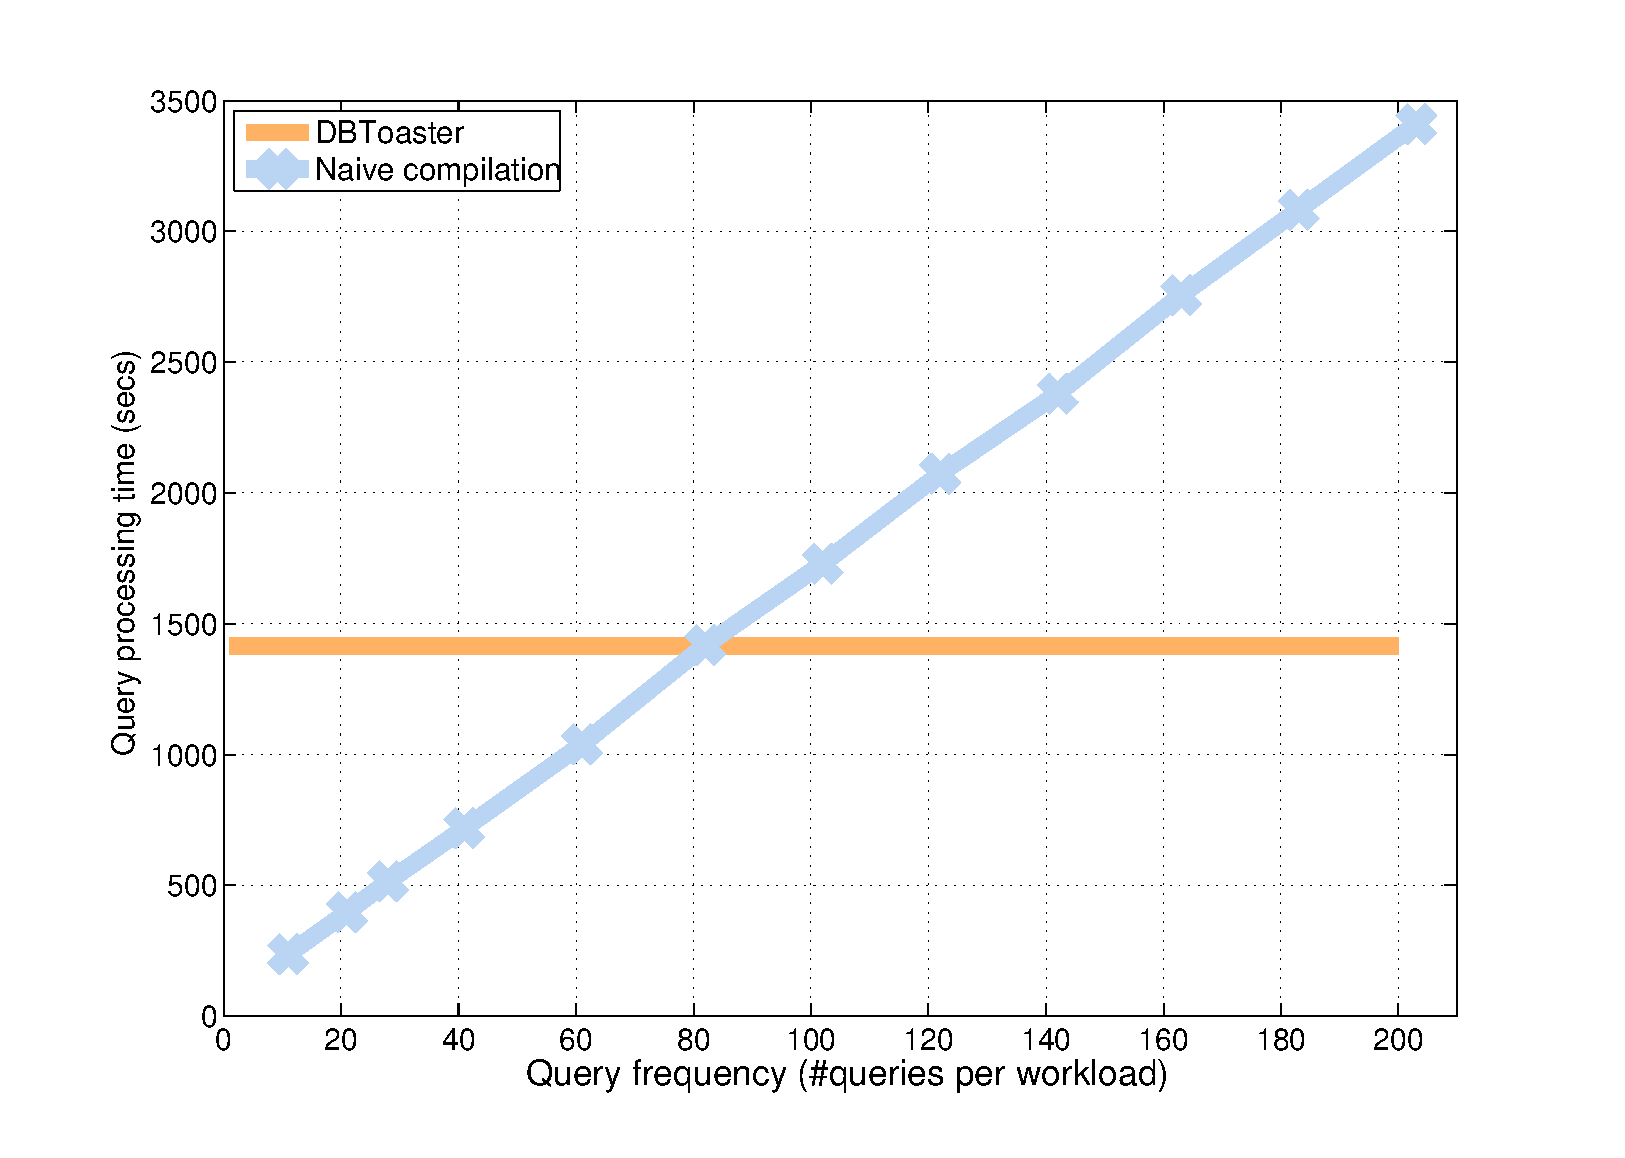
\includegraphics[scale=0.25]{../plots/vwap_query_freq_dn}
\end{center}
\caption{Query frequency limit for VWAP application, indicating the
query execution frequency beyond which DBToaster outperforms the naive query
plan compilation technique.}
\label{fig:vwap_query_freq}
\end{figure}

\begin{figure}
\begin{center}
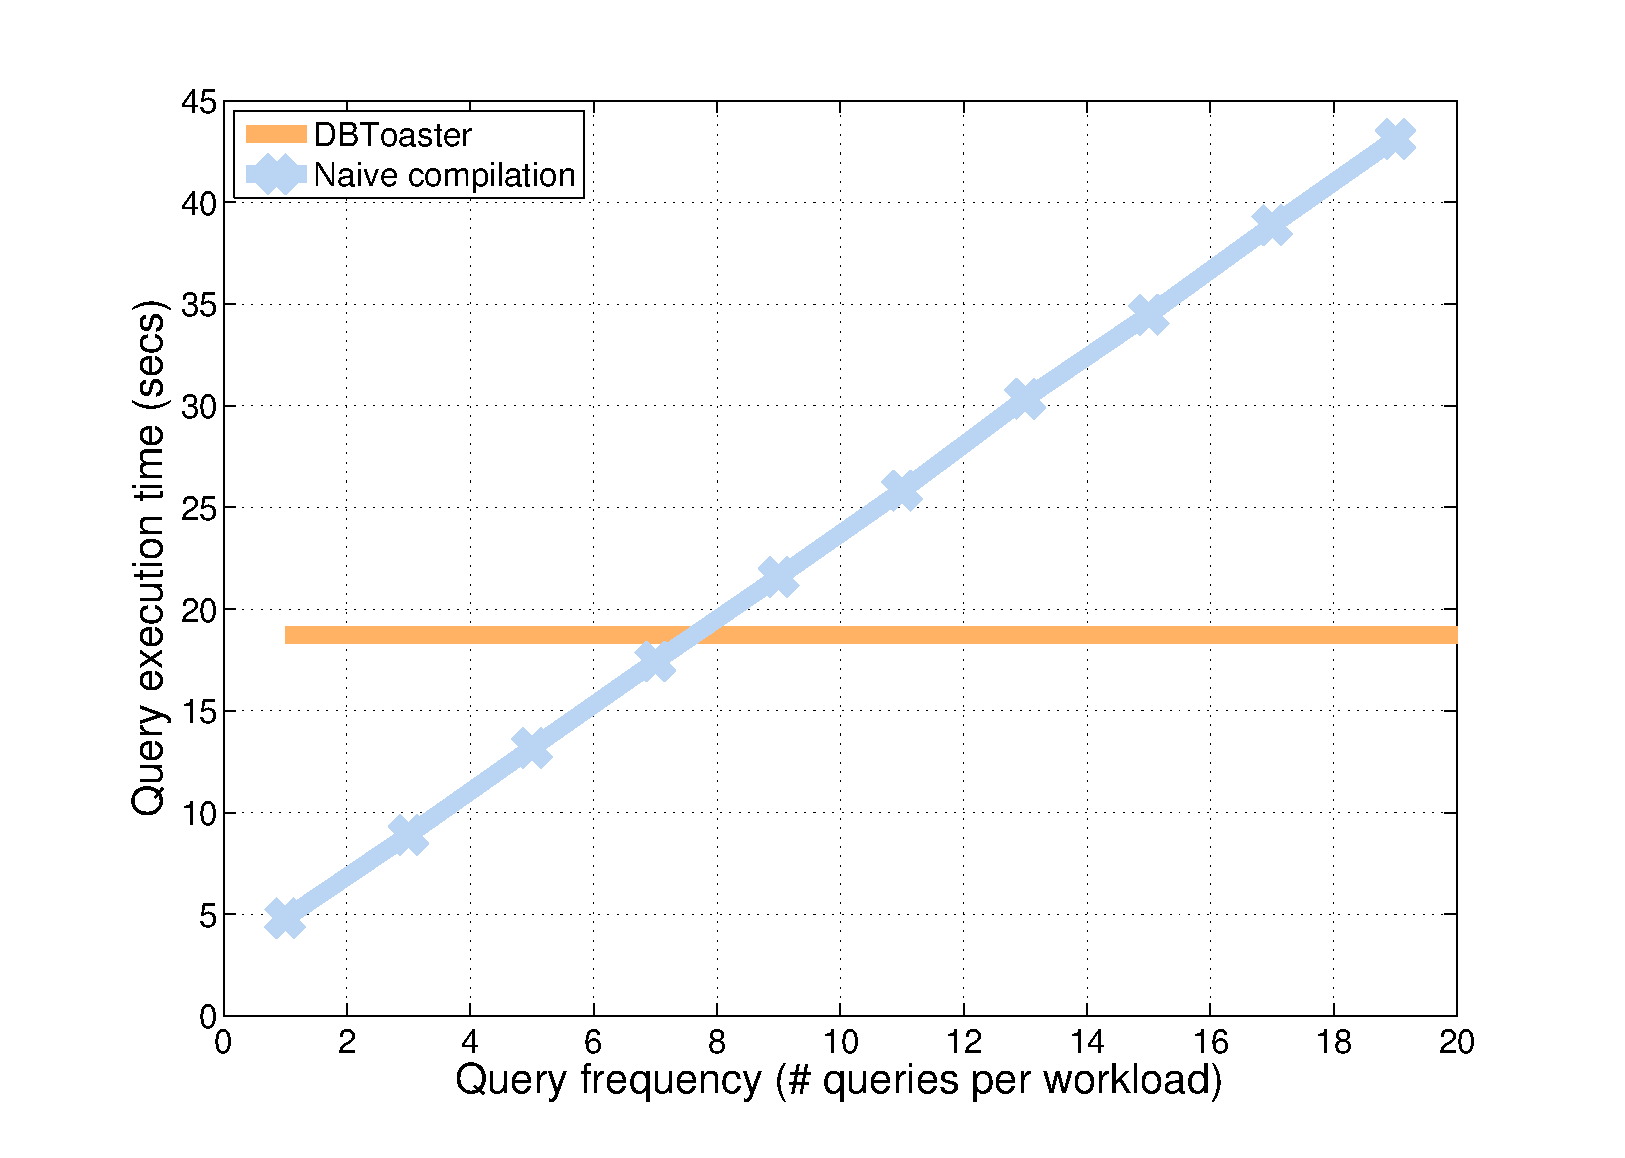
\includegraphics[scale=0.25]{../plots/ssb_query_freq_dn}
\end{center}
\caption{Query frequency limit for warehouse loading application, indicating the
query execution frequency beyond which DBToaster outperforms the naive query
plan compilation technique.}
\label{fig:ssb_query_freq}
\end{figure}

\subsection{Memory Analysis and Batch Execution}


\comment{
Dataset:

\begin{itemize}
  \item TotalView-ITCH dataset: 3 month's worth of MSFT order book messages
  taken from NASDAQ, (~2.2Gb dataset).
  \item Orderbook schema: day, time in us since beginning of day, order id,
  order type, share volume, bid/ask price
\end{itemize}

Queries:

\begin{verbatim}
select * from
  (select ax_bids.mmid, abs(
    sum(ax_bids.volume*
      (act_now.expected_price - ax_bids.price)) -
    sum(ax_asks.volume*
      (ax_asks.price - act_now.expected_price)))
    as ax_bias
  from
    (select mmid, price, volume from bids
       where mmid in axs) as ax_bids,
    (select mmid, price, volume from asks
       where mmid in axs) as ax_asks,
    (select expected_price
        from technical_indicator
        where entrance_condition)
    as act_now
  where ax_bids.mmid = ax_asks.mmid
  group by ax_bids.mmid) as sneaky_ax,
where ax_bias > 10000
\end{verbatim}

Figures:

\begin{enumerate}
  \item Takeaway experiment: end-to-end throughput comparison for a variety of
  insert/update/delete rates. Requires replay speed parameter in data loader.
  Comparison points include Postgres, naive compilation, simple version
  of \compiler, \compiler\ with lazy evaluation, \compiler\ with bulk insert
  mode at 2 or 3 different chunk sizes.

  \item Detail experiment: analyse effect of bulk loading operations compared to
  simple compiler, on a variety of queries, e.g. selectivities and keys.
  Dependent variables for plots: cache hit rates for locality analysis,
  throughput to understand pipelining effects. Is there anything lower lever we
  can do for pipelining?

  \item Detail experiment: selectivity experiment, comparing \compiler\ w/ lazy
  eval, and w/ bulk loading (separately) to next best, for a variety of
  join selectivities and keys.

  \item Detail experiment: space vs recomputation analysis, where we vary the
  maps we keep between extremes of maps from simple decomposition, to full base
  tables.

  \item Quality of compiled code, and compiler effect? e.g. speed provided with
  different -O flags?

\end{enumerate}
}
\section{Related Work}

To the best of our knowledge, there has been limited work addressing the question
of how to compile SQL queries to a low-level imperative language such as C++.
With this in mind, in this section we contrast our map algebra, query rewriting
and execution to several more extensively investigated topics, namely view
maintenance, main-memory databases as well as stream and event processing.

\textbf{View maintenance.}
View maintenance algorithms are in abundance in the database literature, with
topics ranging from efficient view maintenance algorithms given base relation
deltas~\cite{colby-sigmod:96}, which may be eagerly or lazily
applied~\cite{yan-vldb:95,zhou-vldb:07}, to the question of which views to
actually materialize and how to use such views during query
optimization~\cite{kotidis-tods:01,zhou-icde:07}. Zhou et. al~\cite{zhou-vldb:07}
describe a lazy view materialization technique, describing their computation of
deltas starting from a similar point to ours, namely that where a single tuple
has changed as part of a join tree input. However, their approach does not
generalize to the same extent as our map algebra, particularly in the case of
nested aggregations such as the VWAP query seen in this work. Palpanas et.
al.~\cite{palpanas-vldb:02} consider an extension of view maintenance algorithms
to handle non-distributive aggregates, using a selective recomputation strategy
to update only those groups affected by new tuples. More pertinent to the
main-memory database context, Roussopoulos~\cite{roussopoulos-tods:91} presents a
pointer-based (also referred to as an index) approach to implement views with
ViewCache, which incrementally maintains views using algorithms derived from
relational operations. Griffin and Libkin~\cite{griffin-sigmod:95} study the
problem of incremental view maintenance for relations with duplicates, using a
bag algebra for equational reasoning about query operators and to derive update
rules.

Our map expression algebra differs from the issue of view maintenance, in that it
computes a set of maps to support incremental maintenance of a query result,
rather than simply maintaining a single view.
\comment{
Our approach to selecting maps under a memory constraint differs from
traditional cost models to choose views to materialize, given our top-down approach to
decomposing queries with maps.}
Furthermore, given our target application of non-interactive queries and a static
query workload, we need not maintain base relations, unlike standard relational
query processors which do so to provide ad-hoc query capability at the expense of
orders of magnitude performance as seen in our experimental section. This
obviates the need for any pointer or index-based approach to track back to
original base relation tuples, unlike existing main-memory database systems. Most
critically, the notion of compiling these view maintenance algorithms is clearly
a simple and effective technique for generating query executors for unmatched
performance.

\comment{
\begin{itemize}
  \item Asymmetric increment techniques \cite{yang-icde:05}.
  \item Group-by optimizations \cite{yan-icde:94}.
\end{itemize}
\noindent \textbf{DataCubes}
\begin{itemize}
  \item Classical literature \cite{gray-icde:96,mumick-sigmod:97}.
  \item TODO: more papers if we head into cubes.
\end{itemize}
}

\noindent \textbf{Stream and event processing.}
Our work can loosely be compared to complex event and stream processing
engines~\cite{wu-sigmod:06,agrawal-sigmod:08,white-pods:07,motwani-cidr:03,abadi-vldbj:03}
due to the common goal of handling frequently changing data.
SASE+~\cite{agrawal-sigmod:08} and Cayuga~\cite{white-pods:07} are complex event
processors that focus on sequence and pattern query processing on event streams
using NFA-based approaches to process a variety of patterns including Kleene
closures and negation operators. Relational stream processing engines such as
STREAM~\cite{motwani-cidr:03} and Aurora~\cite{abadi-vldbj:03} investigate
continuous query processing architectures that are capable of evaluating
stream-equivalent versions of the standard relation algebra. From the systems
perspective, several novel techniques were developed to address the low-latency,
high-throughput needs of stream applications, including scheduling, load
shedding, and approximate query processing.

Many of these systems are simultaneously addressing the issue of efficiency and
the semantic requirements of their target applications, naturally exploiting
application properties to attain performance. In contrast, our approach is not to
reinvent the wheel in terms of data and query models -- we focus on standard
relational algebra, and an intuitive extension via snapshots and temporal logic,
and purely take on the challenge of designing query executors to best suit a
main-memory environment, arguing for an alternative to plan-based execution.

\comment{
 TODO:
contrast our work to the above -- we avoid the need for windows or punctuations
by making adopting an insert/delete/update stream model, and assuming that the
base relations always fit in memory (i.e. \#deletes/updates is proportional to
\#inserts). Stream processors still evaluate an operator-centric query plan,
hence they cannot exploit compiler optimizations on a query processing kernel
function. They also do not deal with maintaining precomputed partial results as
we do with our map decompositions. What can we say about complex event processors
and the NFAs they evaluate?


\begin{itemize}
  \item STRIP: rule-based maintenance of derived data, with finance app example \cite{adelberg-sigmod:97}
\end{itemize}
}


\noindent \textbf{Compiling high-level languages for embedded systems.}
The embedded systems community has partially studied on compiling high-level
languages into a low-level imperative target language.
Newton et. al.~\cite{newton-lctes:08} present WaveScript, a scripting language
for processing windows, or segments, of a data stream, and describe a compiler to
construct stream dataflow graphs that are capable of running on XScale CPUs.
WaveScript programs are transformed into dataflow graphs, which may in turn be
manipulated by algebraic rewrite rules, similar to a query optimizer. However,
WaveScope does not address relational queries.
Toman and Weddell~\cite{toman-dbtel:01} describe the DEMO system which compiles
SQL queries into Java or C code, implementing query plans as navigational plans
that utilize pointer access in place of scans and indexing, and supporting query
functionality over existing data structures for an embedded program. The authors
use integrity constraints in their compiler to describe the relationship between
schemas and the physical data structures used by an embedded program, and in turn
generate navigational plans and iterators, which can be used to produce C code in
a straightforward manner. DEMO has taken a theoretical approach to describe
their compilation, and does not consider systems issues nor have they released
a prototype and provided an effective tool to perform compilation.


\noindent \textbf{Main memory databases.}
Early work on main-memory databases studied how to reduce the bottleneck effect
of a variety of I/O tasks including recovery tasks such as checkpointing, as well
as logging and locking structures \cite{bohannon-vldb:98,bohannon-sigmod:99}.
There have been several recent efforts on this topic given the developments in
main memory.

Boncz et. al.~\cite{boncz-cidr:05} present the MonetDB/X100 database engine, a
high-performance column-oriented database, that leverages techniques such as
vectorized processing and loop pipelining on chunks of columns while evaluating
operators in query plans. Kallman et. al.~\cite{kallman-pvldb:08} describe
H-Store, a shared-nothing distributed main memory database to provide high
throughput processing on OLTP workloads. H-Store achieves its performance through
careful deployment of horizontally partitioning of relations, and localizing OLTP
transactions to partitions. Raman et. al.~\cite{raman-icde:08} describe Blink, a
row-oriented main memory query processor that extensively uses compression on
denormalized relations, and applies aggregates while scanning these relations as
its main query processing functionality.

These systems span a wide variety of use cases and focus at rearchitecting at a
lower-level than the our approach. For now we have looked at applying a semantic
redesign to describe queries as tuple functions, and reuse much of the work from
the compiler community to provide efficient tuple function execution. Having
applied this first phase to building our runtime, we can now proceed to the
systems level aspects of our tuple functions, for example investigating cache
performance in much greater depth, and in particular understand which of the
above techniques and optimizations can be applied in our context, as well as
leveraging approaches from both the compiler and programming languages
communities in providing compiled query executors.


\section{Conclusions and Future Work}

We have presented \compiler, an SQL compiler, and have demonstrated the
benefits of creating compiled query executors for main-memory processing of
repetitive and standing queries. Our executor is based on the notion of
processing individual tuples, by combining them with aggregated views defined
over the remaining parts of the query. The tuple function is also responsible for
maintaining these aggregate views, and this turns out to be extremely simple and
cheap in the main memory context given our novel map algebra which can readily
convert single tuple deltas into simple arithmetic expressions of parameterized
queries.

Compiled query executors generated by \compiler\ dominate state of the
art database systems, including relational databases and stream processing on a
variety of application scenarios, and is only rivalled in a small set of use
cases by a compiled query executor implementing a plan in its original
operator-centric form. In our view, this raises the possibility that such an
approach should be the de facto processing methodology, as opposed to the
plan-based approach in future query executors.

We view the topic of query compilation and compiled executors as still in its
infancy, and hope that \compiler\ is able to raise interest in this domain. 
As part of ongoing and future work, we plan to investigate the efficiency of
our generated code and understand its memory behavior. A large part of this
includes extending to other non-relational operations in SQL, such as top-k,
and understanding the data structures needed to process tuple functions for
such operations. Furthermore, we would like to apply tuple function
compilation and execution in other novel domains where the database
community is branching out, including scientific databases for executing
simulations, as well as for probabilistic inference on graphical models, where
the common theme in both these domains is a graphical representation of 
computation. Finally the question of getting the right balance of adaptivity
and compilation, especially in light of the difficulty in managing large-scale
database systems, remains an open question. We would like to integrate our
compilation techniques with the emerging techniques for providing self-managing
databases to address this issue.


\comment{
\begin{itemize}
\item
Programming language theory paper: how to compile SQL to use user-specified
data structures.

\item
Compiling down more general declarative languages, with operators and
aggregates whose semantics is definable in the framework. Applications e.g.\
probabilistic inference in graphical models. Compile the graph structure
of the graphical model and the inference algorithms (using e.g.\ mesage
passing techniques) into C code. The data to be processed are the factor
relations/conditional probability tables.

\item
Compiling database applications and the database server together into a single
program that runs robustly and requires no administration. I.e., combine
our query compilation work with automatic administration ideas, if any of
this is actually needed.
\end{itemize}
}

\bibliographystyle{abbrv}
\bibliography{ref}

\appendix

\section{VWAP Query Compilation}

\section{Experimental Workload}

\end{document}
